\documentclass[tikz, margin=2pt]{standalone}
\usepackage[utf8]{inputenc}
\usepackage[T1]{fontenc}

\usepackage{tikz}
\usepackage{helvet}
\usepackage{amsmath}
\usepackage{circuitikz}
\renewcommand\familydefault\sfdefault

\usetikzlibrary{intersections, shapes.arrows, spath3}

\ctikzset {
    logic ports=european,
    logic ports/scale=1.0,
    tripoles/european not symbol=ieee circle,
    resistors/scale=0.7,
    capacitors/scale=0.6,
    diodes/scale=0.6,
}

\begin{document}
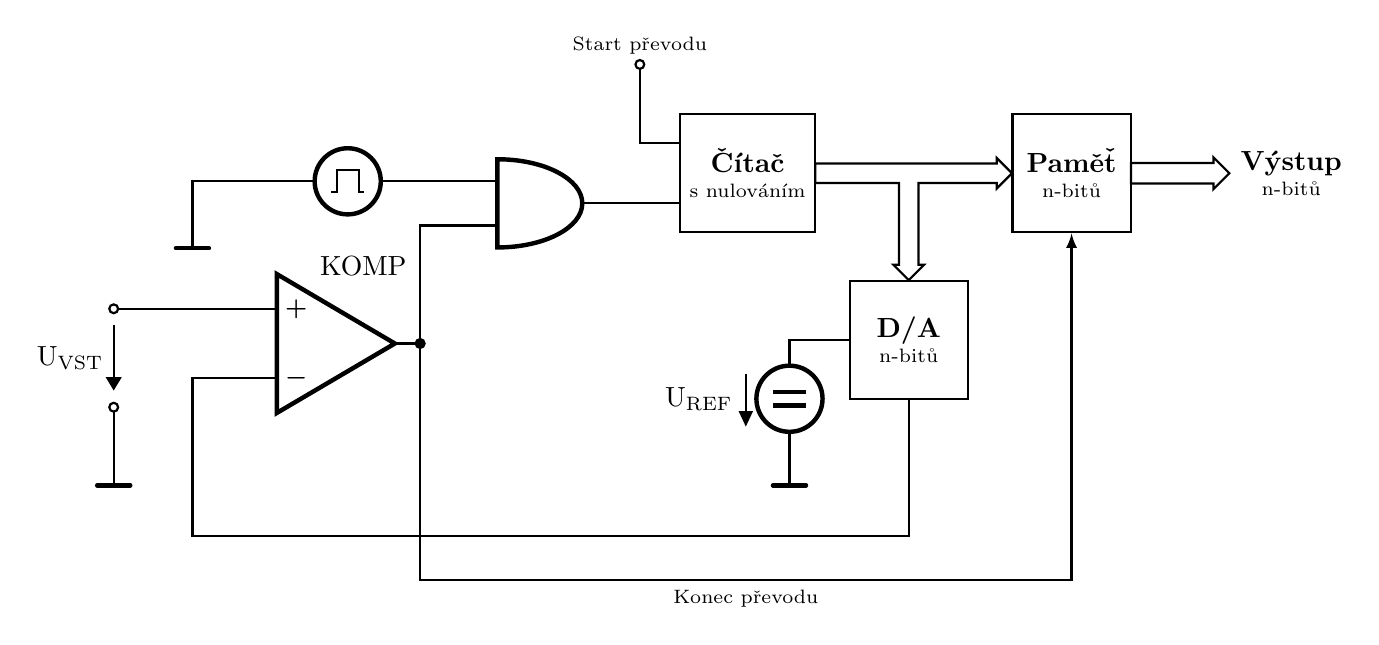
\begin{tikzpicture}[
    straight voltages,
    bus/.style={single arrow, single arrow head extend=2pt},
]

\draw (0, 0) node[bus, minimum height=2.5cm] [spath/save global=a1] (arr) {};
\draw (0, -.1) node[bus, minimum height=1.25cm, rotate=-90, anchor=tail] [spath/save global=a2] (arr2) {};

\tikzset{spath/.cd,
  split at intersections={a1}{a2},
  remove components={a1}{1},
  remove components={a2}{1},
}
\draw[thick, spath/.cd, use=a1, use={a2, weld}, adjust and close=current];
\draw (arr.tail) ++(.5pt, 0) node[draw,thick,  minimum size=1.5cm, align=center, anchor=east] (counter) {\textbf{Čítač}\\[-0.3em] \scriptsize s nulováním};
\draw (arr.tip) ++(-.5pt, 0) node[draw, thick, minimum size=1.5cm, align=center, anchor=west] (mem) {\textbf{Paměť}\\[-0.3em] \scriptsize n-bitů};
\draw (arr2.tip) ++(0, .5pt) node[draw, thick, minimum size=1.5cm, align=center, anchor=north] (dac)  {\textbf{D/A}\\[-0.3em] \scriptsize n-bitů};

\draw (mem.east) ++(-.7pt, 0) node[bus, draw, thick, minimum height=1.25cm, anchor=tail]  (output) {};
\draw (output.tip) node[left, anchor=west, align=center] {\textbf{Výstup}\\[-0.3em] \scriptsize n-bitů};

\draw[thick] ($ (counter.north west)!.75!(counter.south west) $) -- ++(-1, 0) node[and port, anchor=out] (and) {};
\draw[thick] (dac.west) -- ++(-.75, 0) to[dcvsource, v_={ $\text{U}_{\text{REF}} $}] ++(0, -1.5) node[rground] (gnd_ref) {};
\draw[thick] (and.in 2) -- ++(-.75, 0) -- ++(0, -1.5) coordinate (c) node [op amp, noinv input up, anchor=out, scale=.9] (comp) {};
\draw[-latex, thick] (c) node [circ] {} to ++(0, -3) -- node[midway, below] {\scriptsize Konec převodu} (mem.south|-\tikztotarget) -- (mem.south);

\draw[thick] (comp.-) -- ++(-.75, 0) coordinate (to_dac) -- ++(0, -2) -| (dac.south);
\draw[thick] (comp.+) -- ++(-1.75, 0) coordinate (in) node[ocirc] {};
\draw[thick] (in) ++(0, -1.25) coordinate (in_gnd) node[ocirc] {} -- (in_gnd|-gnd_ref) node[rground] {};

\draw[thick] ($ (counter.north west)!.25!(counter.south west) $) -- ++(-.5, 0) -- ++(0, 1) node[ocirc] {} node[above] {\scriptsize Start převodu};

\draw[-{Triangle[scale=1]}, thick] ($(in) +(0, -6pt) $) -- node[midway, left] {$ \text{U}_{\text{VST}} $} ($(in_gnd) +(0, 6pt) $);

\draw[thick] (and.in 1) -- ++(-1.25, 0) node[esourceshape, anchor=right] (clk) {};
\draw[thick] (clk.left) -- (to_dac|-clk.left) -- ++(0, -.5) node[rground] {};
\draw[thick] (clk.center) ++(-6pt, -4pt) -- ++(2pt, 0) -- ++(0, 8pt) -- ++(8pt, 0) -- ++(0, -8pt) -- ++(2pt, 0);

\draw (comp.up) ++(-.25, .5) node[above, right] {KOMP};
\end{tikzpicture}
\end{document}